\documentclass[aspectratio=169]{beamer}

\usetheme{CambridgeUS}
\usecolortheme{seagull}
\setbeamertemplate{navigation symbols}{}

\usepackage[T1]{fontenc}
\usepackage[utf8]{inputenc}
\usepackage{lmodern}
\usepackage{amsmath,amssymb}
\usepackage{xspace}
\usepackage{tikz}

\title[Multi-Interface Networks]{Polylogarithmic Approximation for Covering and Connecting Multi-Interface Networks}
\subtitle{Michal Szyfelbein}
\author{Joint work with Camille Richer}
\institute{Gdansk University of Technology \and Universite Paris-Dauphine}
\date{\today}

% Problem names used throughout slides.
\newcommand{\coverage}{\textsc{Coverage}\xspace}
\newcommand{\connectivity}{\textsc{Connectivity}\xspace}
\newcommand{\OPT}{\mathrm{OPT}}

\begin{document}

\begin{frame}
  \titlepage
\end{frame}

\begin{frame}{Outline}
  \tableofcontents
\end{frame}

\section{Motivation}
\begin{frame}{Motivation}
  \begin{itemize}
    \item In IoT networks, each device may support multiple communication interfaces.
    \item Activating an interface consumes resources (energy, bandwidth, radio time).
    \item Goal: satisfy communication requirements while minimizing the maximum node cost.
  \end{itemize}

  \vspace{0.4em}
  \textbf{Application examples:}
  \begin{itemize}
    \item Heterogeneous smart-home and industrial sensor deployments.
    \item Multi-radio relay/backbone configuration with energy constraints.
  \end{itemize}
\end{frame}

\section{Problem Setup}
\begin{frame}{Graph Model}
  \begin{itemize}
    \item Input graph $G=(V,E)$ represents feasible physical links.
    \item Each vertex $v \in V$ has a set of available interfaces.
    \item Interface activation cost is heterogeneous: depends on both vertex and interface.
    \item Objective (min-max): minimize
    \[
      \max_{v \in V} \; \mathrm{cost}_v.
    \]
  \end{itemize}
\end{frame}

\begin{frame}{Two Optimization Problems}
  \begin{block}{\coverage}
    Activate interfaces so every edge $uv \in E$ is realizable by at least one active interface shared by $u$ and $v$.
  \end{block}

  \begin{block}{\connectivity}
    Given terminal groups, activate interfaces so each group is connected in the induced active subgraph.
  \end{block}

  \vspace{0.5em}
  \textbf{Both use the same min-max objective.}
\end{frame}

\begin{frame}{Illustration: \coverage}
  \centering
  \begin{minipage}[t]{0.49\linewidth}
\centering
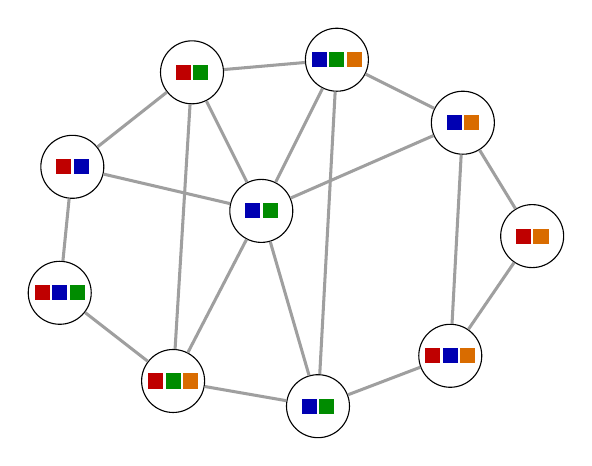
\begin{tikzpicture}[scale=0.80]
    \colorlet{iface1}{red!75!black}
    \colorlet{iface2}{blue!70!black}
    \colorlet{iface3}{green!55!black}
    \colorlet{iface4}{orange!85!black}

    % vertices
    \node[circle, draw, minimum size=8mm, inner sep=0pt] (v1) at (0.0,1.2) {};
    \node[circle, draw, minimum size=8mm, inner sep=0pt] (v2) at (1.9,2.7) {};
    \node[circle, draw, minimum size=8mm, inner sep=0pt] (v3) at (4.2,2.9) {};
    \node[circle, draw, minimum size=8mm, inner sep=0pt] (v4) at (6.2,1.9) {};
    \node[circle, draw, minimum size=8mm, inner sep=0pt] (v5) at (7.3,0.1) {};
    \node[circle, draw, minimum size=8mm, inner sep=0pt] (v6) at (6.0,-1.8) {};
    \node[circle, draw, minimum size=8mm, inner sep=0pt] (v7) at (3.9,-2.6) {};
    \node[circle, draw, minimum size=8mm, inner sep=0pt] (v8) at (1.6,-2.2) {};
    \node[circle, draw, minimum size=8mm, inner sep=0pt] (v9) at (-0.2,-0.8) {};
    \node[circle, draw, minimum size=8mm, inner sep=0pt] (v10) at (3.0,0.5) {};

    % edges
    \draw[gray!75, line width=1.1pt] (v1) -- (v2) -- (v3) -- (v4) -- (v5) -- (v6) -- (v7) -- (v8) -- (v9) -- (v1);
    \draw[gray!75, line width=1.1pt] (v1) -- (v10);
    \draw[gray!75, line width=1.1pt] (v2) -- (v10);
    \draw[gray!75, line width=1.1pt] (v3) -- (v10);
    \draw[gray!75, line width=1.1pt] (v4) -- (v10);
    \draw[gray!75, line width=1.1pt] (v7) -- (v10);
    \draw[gray!75, line width=1.1pt] (v8) -- (v10);
    \draw[gray!75, line width=1.1pt] (v2) -- (v8);
    \draw[gray!75, line width=1.1pt] (v3) -- (v7);
    \draw[gray!75, line width=1.1pt] (v4) -- (v6);

    % available label rectangles in nodes
    \begin{scope}[shift={(v1.center)}]
        \fill[iface1] (-0.26,-0.12) rectangle (-0.02,0.12);
        \fill[iface2] (0.02,-0.12) rectangle (0.26,0.12);
    \end{scope}
    \begin{scope}[shift={(v2.center)}]
        \fill[iface1] (-0.26,-0.12) rectangle (-0.02,0.12);
        \fill[iface3] (0.02,-0.12) rectangle (0.26,0.12);
    \end{scope}
    \begin{scope}[shift={(v3.center)}]
        \fill[iface2] (-0.40,-0.12) rectangle (-0.16,0.12);
        \fill[iface3] (-0.12,-0.12) rectangle (0.12,0.12);
        \fill[iface4] (0.16,-0.12) rectangle (0.40,0.12);
    \end{scope}
    \begin{scope}[shift={(v4.center)}]
        \fill[iface2] (-0.26,-0.12) rectangle (-0.02,0.12);
        \fill[iface4] (0.02,-0.12) rectangle (0.26,0.12);
    \end{scope}
    \begin{scope}[shift={(v5.center)}]
        \fill[iface1] (-0.26,-0.12) rectangle (-0.02,0.12);
        \fill[iface4] (0.02,-0.12) rectangle (0.26,0.12);
    \end{scope}
    \begin{scope}[shift={(v6.center)}]
        \fill[iface1] (-0.40,-0.12) rectangle (-0.16,0.12);
        \fill[iface2] (-0.12,-0.12) rectangle (0.12,0.12);
        \fill[iface4] (0.16,-0.12) rectangle (0.40,0.12);
    \end{scope}
    \begin{scope}[shift={(v7.center)}]
        \fill[iface2] (-0.26,-0.12) rectangle (-0.02,0.12);
        \fill[iface3] (0.02,-0.12) rectangle (0.26,0.12);
    \end{scope}
    \begin{scope}[shift={(v8.center)}]
        \fill[iface1] (-0.40,-0.12) rectangle (-0.16,0.12);
        \fill[iface3] (-0.12,-0.12) rectangle (0.12,0.12);
        \fill[iface4] (0.16,-0.12) rectangle (0.40,0.12);
    \end{scope}
    \begin{scope}[shift={(v9.center)}]
        \fill[iface1] (-0.40,-0.12) rectangle (-0.16,0.12);
        \fill[iface2] (-0.12,-0.12) rectangle (0.12,0.12);
        \fill[iface3] (0.16,-0.12) rectangle (0.40,0.12);
    \end{scope}
    \begin{scope}[shift={(v10.center)}]
        \fill[iface2] (-0.26,-0.12) rectangle (-0.02,0.12);
        \fill[iface3] (0.02,-0.12) rectangle (0.26,0.12);
    \end{scope}
\end{tikzpicture}

\vspace{1mm}
{\scriptsize Available labels}
\end{minipage}
\hfill
\begin{minipage}[t]{0.49\linewidth}
\centering
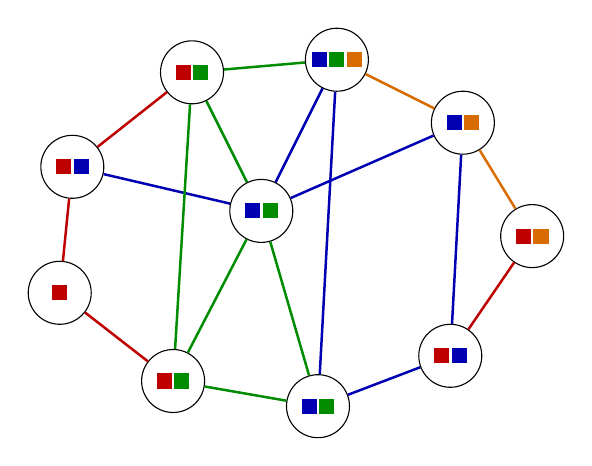
\begin{tikzpicture}[scale=0.80]
    \colorlet{iface1}{red!75!black}
    \colorlet{iface2}{blue!70!black}
    \colorlet{iface3}{green!55!black}
    \colorlet{iface4}{orange!85!black}

    % vertices
    \node[circle, draw, minimum size=8mm, inner sep=0pt] (v1) at (0.0,1.2) {};
    \node[circle, draw, minimum size=8mm, inner sep=0pt] (v2) at (1.9,2.7) {};
    \node[circle, draw, minimum size=8mm, inner sep=0pt] (v3) at (4.2,2.9) {};
    \node[circle, draw, minimum size=8mm, inner sep=0pt] (v4) at (6.2,1.9) {};
    \node[circle, draw, minimum size=8mm, inner sep=0pt] (v5) at (7.3,0.1) {};
    \node[circle, draw, minimum size=8mm, inner sep=0pt] (v6) at (6.0,-1.8) {};
    \node[circle, draw, minimum size=8mm, inner sep=0pt] (v7) at (3.9,-2.6) {};
    \node[circle, draw, minimum size=8mm, inner sep=0pt] (v8) at (1.6,-2.2) {};
    \node[circle, draw, minimum size=8mm, inner sep=0pt] (v9) at (-0.2,-0.8) {};
    \node[circle, draw, minimum size=8mm, inner sep=0pt] (v10) at (3.0,0.5) {};

    % edges colored by covering label
    \draw[iface1, line width=0.9pt] (v1) -- (v2);
    \draw[iface3, line width=0.9pt] (v2) -- (v3);
    \draw[iface4, line width=0.9pt] (v3) -- (v4);
    \draw[iface4, line width=0.9pt] (v4) -- (v5);
    \draw[iface1, line width=0.9pt] (v5) -- (v6);
    \draw[iface2, line width=0.9pt] (v6) -- (v7);
    \draw[iface3, line width=0.9pt] (v7) -- (v8);
    \draw[iface1, line width=0.9pt] (v8) -- (v9);
    \draw[iface1, line width=0.9pt] (v9) -- (v1);
    \draw[iface2, line width=0.9pt] (v1) -- (v10);
    \draw[iface3, line width=0.9pt] (v2) -- (v10);
    \draw[iface2, line width=0.9pt] (v3) -- (v10);
    \draw[iface2, line width=0.9pt] (v4) -- (v10);
    \draw[iface3, line width=0.9pt] (v7) -- (v10);
    \draw[iface3, line width=0.9pt] (v8) -- (v10);
    \draw[iface3, line width=0.9pt] (v2) -- (v8);
    \draw[iface2, line width=0.9pt] (v3) -- (v7);
    \draw[iface2, line width=0.9pt] (v4) -- (v6);

    % selected labels in solution
    \begin{scope}[shift={(v1.center)}]
        \fill[iface1] (-0.26,-0.12) rectangle (-0.02,0.12);
        \fill[iface2] (0.02,-0.12) rectangle (0.26,0.12);
    \end{scope}
    \begin{scope}[shift={(v2.center)}]
        \fill[iface1] (-0.26,-0.12) rectangle (-0.02,0.12);
        \fill[iface3] (0.02,-0.12) rectangle (0.26,0.12);
    \end{scope}
    \begin{scope}[shift={(v3.center)}]
        \fill[iface2] (-0.40,-0.12) rectangle (-0.16,0.12);
        \fill[iface3] (-0.12,-0.12) rectangle (0.12,0.12);
        \fill[iface4] (0.16,-0.12) rectangle (0.40,0.12);
    \end{scope}
    \begin{scope}[shift={(v4.center)}]
        \fill[iface2] (-0.26,-0.12) rectangle (-0.02,0.12);
        \fill[iface4] (0.02,-0.12) rectangle (0.26,0.12);
    \end{scope}
    \begin{scope}[shift={(v5.center)}]
        \fill[iface1] (-0.26,-0.12) rectangle (-0.02,0.12);
        \fill[iface4] (0.02,-0.12) rectangle (0.26,0.12);
    \end{scope}
    \begin{scope}[shift={(v6.center)}]
        \fill[iface1] (-0.26,-0.12) rectangle (-0.02,0.12);
        \fill[iface2] (0.02,-0.12) rectangle (0.26,0.12);
    \end{scope}
    \begin{scope}[shift={(v7.center)}]
        \fill[iface2] (-0.26,-0.12) rectangle (-0.02,0.12);
        \fill[iface3] (0.02,-0.12) rectangle (0.26,0.12);
    \end{scope}
    \begin{scope}[shift={(v8.center)}]
        \fill[iface1] (-0.26,-0.12) rectangle (-0.02,0.12);
        \fill[iface3] (0.02,-0.12) rectangle (0.26,0.12);
    \end{scope}
    \begin{scope}[shift={(v9.center)}]
        \fill[iface1] (-0.12,-0.12) rectangle (0.12,0.12);
    \end{scope}
    \begin{scope}[shift={(v10.center)}]
        \fill[iface2] (-0.26,-0.12) rectangle (-0.02,0.12);
        \fill[iface3] (0.02,-0.12) rectangle (0.26,0.12);
    \end{scope}
\end{tikzpicture}

\vspace{1mm}
{\scriptsize Example covering assignment}
\end{minipage}

\end{frame}

\begin{frame}{Illustration: \connectivity}
  \centering
  % Connection problem illustration – identical topology to problem-illustration.tex.
% Terminals U = {v1, v5, v8} drawn with double circle.
% Steiner vertices used in solution (v4, v10) drawn with dashed border.
% Steiner tree: v1 -[blue]- v10 -[blue]- v4 -[orange]- v5
%                                v10 -[green]- v8
\begin{minipage}[t]{0.49\linewidth}
\centering
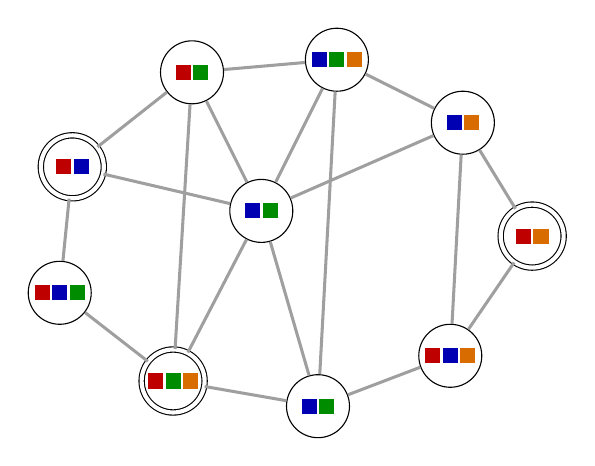
\begin{tikzpicture}[scale=0.80]
    \colorlet{iface1}{red!75!black}
    \colorlet{iface2}{blue!70!black}
    \colorlet{iface3}{green!55!black}
    \colorlet{iface4}{orange!85!black}

    % non-terminal, non-Steiner vertices
    \node[circle, draw, minimum size=8mm, inner sep=0pt] (v2)  at (1.9, 2.7) {};
    \node[circle, draw, minimum size=8mm, inner sep=0pt] (v3)  at (4.2, 2.9) {};
    \node[circle, draw, minimum size=8mm, inner sep=0pt] (v6)  at (6.0,-1.8) {};
    \node[circle, draw, minimum size=8mm, inner sep=0pt] (v7)  at (3.9,-2.6) {};
    \node[circle, draw, minimum size=8mm, inner sep=0pt] (v9)  at (-0.2,-0.8) {};
    % terminal vertices (double circle)
    \node[circle, draw, double, double distance=1.5pt,
          minimum size=8mm, inner sep=0pt] (v1) at (0.0, 1.2) {};
    \node[circle, draw, double, double distance=1.5pt,
          minimum size=8mm, inner sep=0pt] (v5) at (7.3, 0.1) {};
    \node[circle, draw, double, double distance=1.5pt,
          minimum size=8mm, inner sep=0pt] (v8) at (1.6,-2.2) {};
    % Steiner vertices in the solution
    \node[circle, draw, minimum size=8mm, inner sep=0pt] (v4)  at (6.2, 1.9) {};
    \node[circle, draw, minimum size=8mm, inner sep=0pt] (v10) at (3.0, 0.5) {};

    % all edges – thin gray
    \draw[gray!75, line width=1.1pt] (v1) -- (v2) -- (v3) -- (v4) -- (v5) -- (v6) -- (v7) -- (v8) -- (v9) -- (v1);
    \draw[gray!75, line width=1.1pt] (v1) -- (v10);
    \draw[gray!75, line width=1.1pt] (v2) -- (v10);
    \draw[gray!75, line width=1.1pt] (v3) -- (v10);
    \draw[gray!75, line width=1.1pt] (v4) -- (v10);
    \draw[gray!75, line width=1.1pt] (v7) -- (v10);
    \draw[gray!75, line width=1.1pt] (v8) -- (v10);
    \draw[gray!75, line width=1.1pt] (v2) -- (v8);
    \draw[gray!75, line width=1.1pt] (v3) -- (v7);
    \draw[gray!75, line width=1.1pt] (v4) -- (v6);

    % available interface rectangles (identical to problem-illustration.tex)
    \begin{scope}[shift={(v1.center)}]
        \fill[iface1] (-0.26,-0.12) rectangle (-0.02,0.12);
        \fill[iface2] (0.02,-0.12) rectangle (0.26,0.12);
    \end{scope}
    \begin{scope}[shift={(v2.center)}]
        \fill[iface1] (-0.26,-0.12) rectangle (-0.02,0.12);
        \fill[iface3] (0.02,-0.12) rectangle (0.26,0.12);
    \end{scope}
    \begin{scope}[shift={(v3.center)}]
        \fill[iface2] (-0.40,-0.12) rectangle (-0.16,0.12);
        \fill[iface3] (-0.12,-0.12) rectangle (0.12,0.12);
        \fill[iface4] (0.16,-0.12) rectangle (0.40,0.12);
    \end{scope}
    \begin{scope}[shift={(v4.center)}]
        \fill[iface2] (-0.26,-0.12) rectangle (-0.02,0.12);
        \fill[iface4] (0.02,-0.12) rectangle (0.26,0.12);
    \end{scope}
    \begin{scope}[shift={(v5.center)}]
        \fill[iface1] (-0.26,-0.12) rectangle (-0.02,0.12);
        \fill[iface4] (0.02,-0.12) rectangle (0.26,0.12);
    \end{scope}
    \begin{scope}[shift={(v6.center)}]
        \fill[iface1] (-0.40,-0.12) rectangle (-0.16,0.12);
        \fill[iface2] (-0.12,-0.12) rectangle (0.12,0.12);
        \fill[iface4] (0.16,-0.12) rectangle (0.40,0.12);
    \end{scope}
    \begin{scope}[shift={(v7.center)}]
        \fill[iface2] (-0.26,-0.12) rectangle (-0.02,0.12);
        \fill[iface3] (0.02,-0.12) rectangle (0.26,0.12);
    \end{scope}
    \begin{scope}[shift={(v8.center)}]
        \fill[iface1] (-0.40,-0.12) rectangle (-0.16,0.12);
        \fill[iface3] (-0.12,-0.12) rectangle (0.12,0.12);
        \fill[iface4] (0.16,-0.12) rectangle (0.40,0.12);
    \end{scope}
    \begin{scope}[shift={(v9.center)}]
        \fill[iface1] (-0.40,-0.12) rectangle (-0.16,0.12);
        \fill[iface2] (-0.12,-0.12) rectangle (0.12,0.12);
        \fill[iface3] (0.16,-0.12) rectangle (0.40,0.12);
    \end{scope}
    \begin{scope}[shift={(v10.center)}]
        \fill[iface2] (-0.26,-0.12) rectangle (-0.02,0.12);
        \fill[iface3] (0.02,-0.12) rectangle (0.26,0.12);
    \end{scope}
\end{tikzpicture}

\vspace{1mm}
{\scriptsize Available labels (double contour = terminal)}
\end{minipage}
\hfill
\begin{minipage}[t]{0.49\linewidth}
\centering
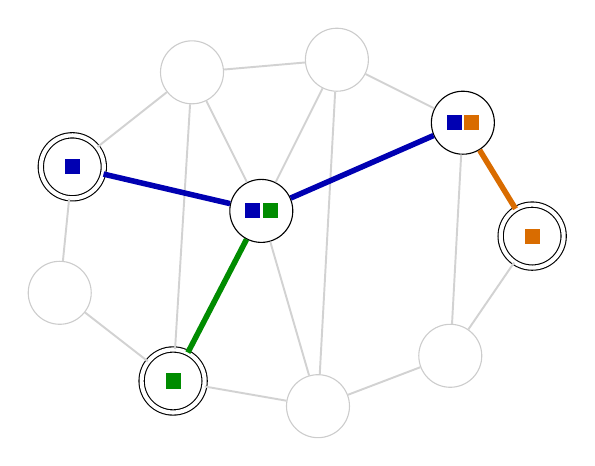
\begin{tikzpicture}[scale=0.80]
    \colorlet{iface1}{red!75!black}
    \colorlet{iface2}{blue!70!black}
    \colorlet{iface3}{green!55!black}
    \colorlet{iface4}{orange!85!black}

    % non-terminal, non-Steiner vertices (faded)
    \node[circle, draw=gray!40, minimum size=8mm, inner sep=0pt] (v2)  at (1.9, 2.7) {};
    \node[circle, draw=gray!40, minimum size=8mm, inner sep=0pt] (v3)  at (4.2, 2.9) {};
    \node[circle, draw=gray!40, minimum size=8mm, inner sep=0pt] (v6)  at (6.0,-1.8) {};
    \node[circle, draw=gray!40, minimum size=8mm, inner sep=0pt] (v7)  at (3.9,-2.6) {};
    \node[circle, draw=gray!40, minimum size=8mm, inner sep=0pt] (v9)  at (-0.2,-0.8) {};
    % terminal vertices (double circle)
    \node[circle, draw, double, double distance=1.5pt,
          minimum size=8mm, inner sep=0pt] (v1) at (0.0, 1.2) {};
    \node[circle, draw, double, double distance=1.5pt,
          minimum size=8mm, inner sep=0pt] (v5) at (7.3, 0.1) {};
    \node[circle, draw, double, double distance=1.5pt,
          minimum size=8mm, inner sep=0pt] (v8) at (1.6,-2.2) {};
    % Steiner vertices used in solution
    \node[circle, draw, minimum size=8mm, inner sep=0pt] (v4)  at (6.2, 1.9) {};
    \node[circle, draw, minimum size=8mm, inner sep=0pt] (v10) at (3.0, 0.5) {};

    % non-tree edges (thin, faded)
    \draw[gray!35, line width=0.7pt] (v1) -- (v2) -- (v3) -- (v4) -- (v5) -- (v6) -- (v7) -- (v8) -- (v9) -- (v1);
    \draw[gray!35, line width=0.7pt] (v2) -- (v10);
    \draw[gray!35, line width=0.7pt] (v3) -- (v10);
    \draw[gray!35, line width=0.7pt] (v7) -- (v10);
    \draw[gray!35, line width=0.7pt] (v2) -- (v8);
    \draw[gray!35, line width=0.7pt] (v3) -- (v7);
    \draw[gray!35, line width=0.7pt] (v4) -- (v6);

    % Steiner tree edges (thick, coloured by activated interface)
    \draw[iface2, line width=2.0pt] (v1)  -- (v10); % iface2 (blue)
    \draw[iface2, line width=2.0pt] (v10) -- (v4);  % iface2 (blue)
    \draw[iface4, line width=2.0pt] (v4)  -- (v5);  % iface4 (orange)
    \draw[iface3, line width=2.0pt] (v10) -- (v8);  % iface3 (green)

    % assigned interfaces (solution only)
    \begin{scope}[shift={(v1.center)}]
        \fill[iface2] (-0.12,-0.12) rectangle (0.12,0.12);
    \end{scope}
    \begin{scope}[shift={(v4.center)}]
        \fill[iface2] (-0.26,-0.12) rectangle (-0.02,0.12);
        \fill[iface4] (0.02,-0.12) rectangle (0.26,0.12);
    \end{scope}
    \begin{scope}[shift={(v5.center)}]
        \fill[iface4] (-0.12,-0.12) rectangle (0.12,0.12);
    \end{scope}
    \begin{scope}[shift={(v8.center)}]
        \fill[iface3] (-0.12,-0.12) rectangle (0.12,0.12);
    \end{scope}
    \begin{scope}[shift={(v10.center)}]
        \fill[iface2] (-0.26,-0.12) rectangle (-0.02,0.12);
        \fill[iface3] (0.02,-0.12) rectangle (0.26,0.12);
    \end{scope}
\end{tikzpicture}

\vspace{1mm}
{\scriptsize Example connecting assignment}
\end{minipage}

\end{frame}

\begin{frame}{Preprocessing (from the paper)}
  \begin{itemize}
    \item \textbf{Scaling of costs:} test consecutive powers of $2$ and guess the smallest $b$ such that the optimal solution uses interfaces of cost at most $2^b$.
    \item Discard interfaces with cost larger than $2^b$ and divide all remaining costs by $2^b$.
    \item After scaling: costs are in $[0,1]$ and (for the right guess) $\OPT \ge 1/2$.
    \item \textbf{Cheap vs expensive vertices:}
    \item If $\sum_{i\in\lambda(v)} c(i,v) \le 1$, vertex $v$ is cheap and we can activate all interfaces at $v$.
    \item Otherwise $v$ is expensive, and we assume in solutions that
    \[
      \sum_{i\in\lambda(v)} c(i,v)\,x_{i,v} \ge 1.
    \]
  \end{itemize}
\end{frame}

\section{Main Results}
\begin{frame}{Main Approximation Guarantees}
  \begin{itemize}
    \item \coverage with heterogeneous costs:
    \[
      O(\log m)\text{-approximation}
    \]
    via LP relaxation + randomized rounding.

    \item Simpler deterministic rounding for \coverage:
    \[
      k\text{-approximation}
    \]
    where $k$ is the number of interfaces.

    \item \connectivity with heterogeneous costs:
    \[
      O(\log^2 m)\text{-approximation}
    \]
    via LP with flow/cut constraints + iterative randomized rounding.
  \end{itemize}
\end{frame}

\section{Techniques}
\begin{frame}{Technique 1: ILP for \coverage (paper formulation)}
  \small
  Variables: $x_{i,v}\in\{0,1\}$ and objective variable $M$.

  \begin{align*}
    \min\quad & M\\
    \text{s.t.}\quad
    & \sum_{i\in\lambda(v)} c(i,v)\,x_{i,v} \le M && \forall v\in V,\\
    & \sum_{i\in\lambda(u)\cap\lambda(v)} \min\{x_{i,u},x_{i,v}\} \ge 1 && \forall uv\in E,\\
    & \begin{cases}
      x_{i,v}=1\ \forall i\in\lambda(v) & \text{if } \sum_{i\in\lambda(v)} c(i,v)\,x_{i,v}<1,\\
      \sum_{i\in\lambda(v)} c(i,v)\,x_{i,v}\ge 1 & \text{otherwise}
    \end{cases} && \forall v\in V,\\
    & x_{i,v}\in\{0,1\} && \forall v\in V,\ i\in\lambda(v).
  \end{align*}
  \normalsize
  Non-linearity is in the $\min\{x_{i,u},x_{i,v}\}$ term; in the paper it is linearized with variables $z_{i,uv}$.
\end{frame}

\begin{frame}{Technique 2: ILP for \connectivity (paper formulation)}
  \small
  Variables: $x_{i,v}\in\{0,1\}$, $y_{uv}\in\{0,1\}$, objective variable $M$.

  \begin{align*}
    \min\quad & M\\
    \text{s.t.}\quad
    & \sum_{i\in\lambda(v)} c(i,v)\,x_{i,v} \le M && \forall v\in V,\\
    & \sum_{i\in\lambda(u)\cap\lambda(v)} \min\{x_{i,u},x_{i,v}\} \ge y_{uv} && \forall uv\in E,\\
    & \begin{cases}
      x_{i,v}=1\ \forall i\in\lambda(v) & \text{if } \sum_{i\in\lambda(v)} c(i,v)\,x_{i,v}<1,\\
      \sum_{i\in\lambda(v)} c(i,v)\,x_{i,v}\ge 1 & \text{otherwise}
    \end{cases} && \forall v\in V,\\
    & y(\delta(S))\ge 1 && \forall r\in[p],\ \forall S\subset V:\ S\cap U_r\neq\emptyset,\ (V\setminus S)\cap U_r\neq\emptyset,\\
    & x_{i,v}\in\{0,1\},\ y_{uv}\in\{0,1\}.
  \end{align*}
  \normalsize
  The LP relaxation is solved with a separation oracle for cut constraints.
\end{frame}

\begin{frame}{Pseudocode: Randomized Algorithm for \coverage}
  \textbf{Input:} LP-relaxed solution $\{x_{i,v}\}_{i\in\lambda(v),\,v\in V}$.

  \vspace{0.4em}
  \textbf{Procedure}
  \begin{enumerate}
    \item Pick independent uniformly random thresholds $t_i\in(0,1)$ for each $i\in[k]$.
    \item For every $v\in V$, set
    \[
      \lambda_A(v) \gets \{i\in\lambda(v):\ 3\ln m\cdot x_{i,v} \ge t_i\}.
    \]
    \item Return $\{\lambda_A(v)\}_{v\in V}$.
  \end{enumerate}
\end{frame}

\begin{frame}{Pseudocode: Iterative Algorithm for \connectivity}
  \textbf{Input:} LP-relaxed solution $\{x_{i,v}\},\{y_{uv}\}$.

  \vspace{0.4em}
  \textbf{Procedure}
  \begin{enumerate}
    \item For every edge $e\in E$, set $p_e\gets\min\{1,4\ln m\cdot y_e\}$ and sample $Y_e\in\{0,1\}$ with $\Pr[Y_e=1]=p_e$.
    \item Let $H$ be the subgraph induced by edges with $Y_e=1$.
    \item Initialize $\lambda_A(v)\gets\emptyset$ for all $v\in V$ and $j\gets 1$.
    \item While $\mathrm{cov}(\lambda_A,H)\neq E(H)$:
    \begin{itemize}
      \item Pick independent uniformly random thresholds $t_i\in(0,1)$ for each $i\in[k]$.
      \item Set $\lambda_A^j(v)\gets\{i\in\lambda(v): x_{i,v}\ge t_i\}$ for every $v\in V$.
      \item Update $\lambda_A\gets\lambda_A\cup\lambda_A^j$ and $j\gets j+1$.
    \end{itemize}
    \item Return $\lambda_A$.
  \end{enumerate}
\end{frame}

\begin{frame}{Proof Outline for \coverage: Main Claims}
  \begin{block}{Lemma 1 (Feasibility)}
    For any edge $uv$, $\Pr[\lambda_A(u)\cap\lambda_A(v)=\emptyset]\le 1/m^3$.
    By union bound over all $m$ edges, Algorithm 1 returns a covering assignment with probability at least $1-1/m^2$.
  \end{block}

  \begin{block}{Lemma 2 (Cost)}
    For each expensive vertex $v$, $\mathbb{E}[\mathrm{cost}(v,\lambda_A)]\le 3\ln m\cdot \sum_{i\in\lambda(v)}x_{i,v}c(i,v)$.
    Chernoff with $\delta=2$ gives
    \[
      \Pr\!\left[\mathrm{cost}(v,\lambda_A)\ge 9\ln m\cdot\sum_{i\in\lambda(v)}x_{i,v}c(i,v)\right]\le 1/m^3.
    \]
    Union bound over vertices gives cost at most $9\ln m\cdot\OPT$ with high probability.
  \end{block}

  Combining the two lemmas yields the $O(\log m)$-approximation theorem.
\end{frame}

\begin{frame}{Proof Outline for \connectivity: Main Claims}
  \begin{block}{Lemma 1 (Terminal connectivity in sampled graph $H$)}
    With high probability, for every terminal group $U_r$, graph $H$ connects all terminals in $U_r$.
    Proof uses cut constraints, Karger's bound on near-min cuts, and union bound.
  \end{block}

  \begin{block}{Lemma 2 (Progress per iteration)}
    If $H_j$ is the uncovered part of $H$ at iteration $j$, then
    \[
      \mathbb{E}\big[|\mathrm{cov}(\lambda_A^j,H_j)|\big]
      \ge \frac{1-1/e}{4\ln m}\cdot \mathbb{E}\big[|E(H_j)|\big].
    \]
  \end{block}

  Next: iteration bound and final cost bound.
\end{frame}

\begin{frame}{Proof Outline for \connectivity: Main Claims (cont.)}
  \begin{block}{Lemmas 3--5 (Iterations and cost)}
    Number of iterations $I$ satisfies
    \[
      \mathbb{E}[I]\le \frac{9\ln^2 m}{1-1/e},
      \qquad
      \Pr\!\left[I\ge \frac{9\ln^2 m}{1-1/e}\right]\le \frac{1}{m}.
    \]
    With high probability,
    \[
      \mathrm{cost}(\lambda_A)\le \frac{27\ln^2 m}{1-1/e}\cdot \OPT.
    \]
  \end{block}

  Therefore Algorithm 3 is an $O(\log^2 m)$-approximation with high probability.
\end{frame}

\section{Context and Impact}
\begin{frame}{How This Compares to Prior Work}
  \begin{itemize}
    \item Prior logarithmic guarantees were largely for homogeneous settings.
    \item This work handles heterogeneous costs directly.
    \item Provides the first non-trivial approximation for heterogeneous group connectivity under min-max objective.
  \end{itemize}
\end{frame}

\begin{frame}{Limitations and Open Questions}
  \begin{itemize}
    \item Can $O(\log^2 m)$ for \connectivity be improved to $O(\log m)$?
    \item Tight lower bounds in the heterogeneous setting.
    \item Derandomization possibilities for the best guarantees.
    \item Practical performance vs. worst-case theory.
  \end{itemize}
\end{frame}

\section{Backup}
\begin{frame}{Backup: Notation}
  \begin{itemize}
    \item $n = |V|$, $m = |E|$, $k =$ number of interfaces.
    \item $c_{v,i}$: cost of activating interface $i$ at vertex $v$.
    \item $\OPT$: optimal min-max value.
  \end{itemize}
\end{frame}

\begin{frame}{Backup: Candidate Theorem Slide}
  \textbf{Theorem (placeholder).}

  \vspace{0.5em}
  For every instance of \coverage, the algorithm returns a feasible solution of value at most
  \[
    O(\log m)\cdot \OPT.
  \]

  \vspace{0.5em}
  \textbf{Proof sketch placeholder:}
  \begin{itemize}
    \item LP feasibility at guessed threshold.
    \item Concentration bound for all edge constraints.
    \item Union bound over edges.
  \end{itemize}
\end{frame}

\begin{frame}
  \centering
  {\Huge Thank you!}

  \vspace{1em}
  Questions?
\end{frame}

\end{document}
